 \documentclass[11pt]{article}

%\usepackage{setspace}
%\documentclass[final,leqno]{siamltex}
\usepackage{smoothing_paper}



\usepackage[section]{placeins}
\usepackage{tabularx,ragged2e,booktabs,caption}

%%%%%%%%%%%%%%%%%%%%%%%%%%%%%%%%chiheb commands


%%%%%%%%%%%%%%%%%
\newcommand{\ie}{\emph{i.e.}}
\newcommand{\eg}{\emph{e.g.}}
\newcommand{\cf}{\emph{cf.}}
\newcommand{\prob}[1]{\mathrm{P}\left(#1\right)}
\newcommand{\expt}[1]{\mathrm{E}\left[#1\right]}
\newcommand{\expth}[1]{\hat{\mathrm{E}}\left[#1\right]}



\newcommand{\rset}{\mathbb{R}}
\newcommand{\nset}{\mathbb{N}}
\newcommand{\zset}{\mathbb{Z}}



\newcommand{\PERIOD}{.}
\newcommand{\COMMA}{,}
\newcommand{\BIGSPACE}{\,\,\,\,\,\,\,}



\newcommand{\Ordo}[1]{{\mathcal{O}}\left(#1\right)}
\newcommand{\ordo}[1]{{o}\left(#1\right)}

%%%%%%%%%%%%%%%%%%%%%%%%%%%%%%%%%%%%%%%%%%%%%%%%%%%%%%%%%%%%%%%%%%%%%%%%
%%
%% DO WE RELLY NEED THE FOLLOWING??

%%  new margin
%%%%%%%%%%%%%%%%%%%%%%%%%%%%%%%%%%%%%%%%%%%
\pagestyle{plain}                                                      %%
%%%%%%%%%% EXACT 1in MARGINS %%%%%%%                                   %%
\setlength{\textwidth}{6.5in}     %%                                   %%
\setlength{\oddsidemargin}{0in}   %%   
\setlength{\evensidemargin}{0in}  %%        
\setlength{\textheight}{8.5in}    %%       
\setlength{\topmargin}{-0.2in}    %%   
\setlength{\headheight}{0in}      %%    
\setlength{\headsep}{0in}         %%                   
\setlength{\footskip}{.5in}       %%                       
%%%%%%%%%%%%%%%%%%%%%%%%%%%%%%%%%%%%                                   %%
\newcommand{\required}[1]{\section*{\hfil #1\hfil}}                    %%
\renewcommand{\refname}{\hfil References Cited\hfil}                   %%

\def\SMALLSKIP{\smallskip}
\def\MEDSKIP{\medskip}
\def\BIGSKIP{\bigskip}

%%
%%%%%%%%%%%%%%%%%%%%%%%%%%%%%%%%%%%%%%%%%%%%%%%%%%%%%%%%%%%%%%%%%%%%%

\makeatletter
\def\BState{\State\hskip-\ALG@thistlm}
\makeatother



%%%%%%%%%%%%%%%%%%%%%%%%%%%%%%%%%%%%%%%%

\title{Comparing the results of Cholesky and Hybrid schemes for the rBergomi } 




%\doublespacing
\begin{document}
\maketitle







%\pagestyle{myheadings}
\thispagestyle{plain}

\setcounter{tocdepth}{1}

%\section{Intoduction}\label{sec:Intoduction}
%There are mainly two point that we want to improve comparing to the current version of the rBergomi manuscript:

\begin{itemize}
\item[i)]  Some internal beliefs that maybe we are making wrong assumptions about the asymptotic rates of convergence for the weak error, when using the Hybrid scheme. Therefore, we suggest to test the first case of parameters with Cholesky scheme (See Section \ref{sec:Details of Cholesky scheme coupled with hierarchical reresentation} for details about Cholesky scheme). 

\begin{itemize}
\item If we find similar results as observed with the hybrid scheme then we may add just a remark or the results of Cholesky for that case. Otherwise, we may repeat all experiments, or change the used hierarchical representation. 
\item It is critical also to check if the hierarchical representation is working for the Cholesky scheme as we observed in the case of the hybrid scheme. In fact, for the hybrid scheme it was clear that $\mathbf{W}^{(1)}$ dimensions are more important than those of $\mathbf{W}^{(2)}$, reducing already  the effective dimension from $2N$ to $N$, before even that the Brownian bridge construction creates more anisotropy for  $\mathbf{W}^{(1)}$ directions. However, in the Cholesky scheme, we do not have this obvious distinction.
\end{itemize}
\item[ii)]Provide some errors bounds for the quadrature error of MISC (See Section \ref{sec:MISC error estimate} for details). This will make the method more robust and more convincing in terms of practical use. In fact, at the current stage, the errors that we provide are functions of $\text{TOL}_{\text{MISC}}$, that is $ \mathcal{E}_Q(\text{TOL}_{\text{MISC}},N)=f(\text{TOL}_{\text{MISC}})$ and it is not clear to us the behavior of $f$.

There are two ways to achieve this:

\begin{enumerate}
\item The first way relies on estimating the interpolation error and then by Monte Carlo deduce the quadrature error. We believe that the Monte Carlo error will be dominated by the statistical error and we need maybe few samples for its estimation. For this purpose, we will use the code provided by Joakim.  

\item The second way will be an alternative for the first way in case we failed to have nice error bounds. It is more expensive but more reliable. It is based on learning the error curve which will be parameterized by the different parameters involved in the pricing problem under the rough Bergomi model in addition to MISC tolerance, $\text{TOL}_{\text{MISC}}$, and the number of time steps, $N$.
\end{enumerate}




\end{itemize}


 \section{Problem setting}\label{sec:Problem setting}

\subsection{The rBergomi model}\label{sec:The rBergomi model}

We consider the rBergomi model for the price process $S_t$, normalized to $r=0$\footnote{$r$ is the interest rate.}, which is defined by

\begin{align}\label{eq:rBergomi_model1}
	dS_t &= \sqrt{v_t} S_t dZ_t, \nonumber \\
	v_t &= \xi_0(t) \exp\left( \eta \widetilde{W}_t^H - \frac{1}{2} \eta^2 t^{2H} \right),
\end{align}
where the Hurst parameter $0 < H < 1$  and  $\eta>0$. We refer to $v_t$ as the variance process, and $\xi_0(t) = \expt{v_t}$ is  the forward variance curve.  Here, $\widetilde{W}^H $ is a certain Riemann-Liouville fBm
process\footnote{The so-called Riemann-Liouville processes are deduced from the standard Brownian motion by applying Riemann-Liouville fractional operators, whereas the standard fBm requires a weighted fractional operator.},  defined by
\begin{align}\label{eq:Volterra process}
	\widetilde{W}_t^H = \int_0^t K^H(t,s) dW_s^1, \quad t \ge 0 \COMMA
\end{align}
where the kernel $K^H : \rset_+ \times \rset_+ \rightarrow \rset_+$ is
\begin{equation*}
 \quad K^H(t,s) = \sqrt{2H} (t-s)^{H - 1/2},\quad \forall \: 0 \le s \le t.
\end{equation*}
By construction, $\widetilde{W}^H $ is a centered, locally $(H-\epsilon)$- H\"older continuous, Gaussian process with $\text{Var}\left[\widetilde{W}^H_t \right] = t^{2H}$, and a dependence structure defined by 
 \begin{equation*}
 \expt{\widetilde{W}^H_u  \widetilde{W}^H_v}=u^{2H} G\left(\frac{v}{u} \right),\quad v >u \COMMA
 \end{equation*}
 where for $x \ge 1$ and $\gamma=\frac{1}{2}-H$
 
  \begin{equation*}
G(x)=2H \int_{0}^1 \frac{ds}{(1-s)^{\gamma} (x-s)^{\gamma}}.
 \end{equation*}
In \eqref{eq:rBergomi_model1} and \eqref{eq:Volterra process}, $W^1, Z$ denote two \emph{correlated} standard Brownian motions with correlation $\rho \in ]-1,0]$, so that we can represent $Z$ in terms of $W^1$ as
\begin{align*}
	Z=\rho	W^1+ \bar{\rho}W^\perp = \rho W^1+\sqrt{1-\rho^2} W^\perp,
\end{align*}
where $(W^1,W^\perp)$ are two independent standard Brownian motions.
Therefore, the solution to \eqref{eq:rBergomi_model1}, with $S(0)=S_0$, can be written as 

\begin{align}\label{eq:rBergomi_model}
	S_t&= S_0  \operatorname{exp}\left( \int_{0}^{t} \sqrt{v(s)} dZ(s)- \frac{1}{2} \int_{0}^{t} v(s) ds   \right),\quad S_0>0 \nonumber\\
	v_u&=\xi_0(u) \operatorname{exp}\left( \eta \widetilde{W}_u^H- \frac{\eta^2}{2} u^{2H} \right), \quad \xi_0>0 \PERIOD
\end{align}
The filtration $(\mathcal{F}_t)_{t\ge 0}$ can here be taken as the one generated by the two-dimensional Brownian motion $(W^1,W^\perp)$ under the risk neutral measure $\mathbb{Q}$, resulting in  a filtered probability space $(\Omega,\mathcal{F}, \mathcal{F}_t,\mathbb{Q})$. The stock price process $S$ is clearly then a local
$(\mathcal{F}_t)_{t\ge 0}$-martingale and a supermartingale.  We shall henceforth use the notation $\expt{.} = E^{\mathbb{Q}}\left[. \mid \mathcal{F}_0\right]$ unless we state otherwise.




\subsection{Simulation of the rBergomi model}\label{sec:Simulation of the rBergomi model}

One of the numerical challenges encountered in the simulation of the rBergomi dynamics  is the computation of  $\int_{0}^{T} \sqrt{v_t} dW_t^1$ and $V=\int_{0}^{T} v_t dt$ in \eqref{BS_formula_rbergomi}, mainly because of the singularity of the Volterra kernel $K^H(s,t)$ at the diagonal $s = t$. In fact,  one needs to jointly simulate two Gaussian processes $(W_t^1, \widetilde{W}^H_t: 0 \le t \le T)$, resulting in $W^1_{t_1},\dots, W^1_{t_N}$ and $\widetilde{W}^H_{t_1},\dots, \widetilde{W}^H_{t_N}$ along a given time grid $t_1 <\dots < t_N$. In the literature, there are essentially two suggested ways to achieve this:
 \begin{enumerate}
% 	\item[i)] \textbf{Simple Euler discretization}: Euler discretization of the integral \eqref{eq:Volterra process}, defining $\widetilde{W}^H$, together with classical simulation of increments of $W^1$. This is inefficient because the integral is singular and adaptivity may not improve the scheme since the singularity moves with time. For this method, we need an $N$-dimensional random Gaussian input vector to produce one (approximate, inaccurate) sample of $W^1_{t_1},\dots, W^1_{t_N}, \widetilde{W}^H_{t_1},\dots, \widetilde{W}_{t_N}$.
 	
 	\item[i)] \textbf{Covariance based approach}: Given that $W^1_{t_1},\dots, W^1_{t_N}, \widetilde{W}^H_{t_1},\dots, \widetilde{W}_{t_N}$ together form a ($2N$)-dimensional Gaussian random vector with computable covariance matrix, one can use Cholesky decomposition of the covariance matrix to produce exact samples of $W^1_{t_1},\dots, W^1_{t_N}, \linebreak \widetilde{W}^H_{t_1},\dots, \widetilde{W}_{t_N}$ from $2 N$-dimensional Gaussian random vector as  input. This method is exact but slow. The simulation  requires $\Ordo{N^2}$ flops. Note that the offline cost is $\Ordo{N^3}$ flops.
 	
 	\item[ii)]  \textbf{The hybrid scheme}: This scheme uses a different approach, which is essentially based on  Euler discretization  but crucially improved by moment
 	matching for the singular term in the left point rule. It is also
 	inexact in the sense that samples produced here do not exactly have the distribution of $W^1_{t_1},\dots, W^1_{t_N}, \widetilde{W}^H_{t_1},\dots, \widetilde{W}_{t_N}$, however they are much more accurate than samples produced from simple Euler discretization, but much faster than method $(i)$. As in method $(i)$, in this case, we need a $2 N$-dimensional Gaussian random input vector to produce one 	sample of $W^1_{t_1},\dots, W^1_{t_N}, \widetilde{W}^H_{t_1},\dots, \widetilde{W}_{t_N}$.
 \end{enumerate}

In this work, we adopt approach  $(ii)$ for the simulation of the rBergomi dynamics. The hybrid scheme discretizes the  $\widetilde{W}^H$ process into Wiener integrals of power functions and a Riemann sum, appearing from approximating the kernel by power functions near the origin and step functions elsewhere (see \eqref{eq:Hybrid_scheme}). We utilize the hybrid scheme with $\kappa=1$\footnote{There are different variants of the hybrid scheme depending on the value of $\kappa$.}, which is based on the following approximation
\begin{align}\label{eq:Hybrid_scheme}
\widetilde{W}^H_{\frac{i}{N}} \approx \bar{W}^H_{\frac{i}{N}}&= \sqrt{2H} \left(  W^2_i+\sum_{k=2}^{i} \left(\frac{b_k}{N}\right)^{H-\frac{1}{2}} \left(W_{\frac{i-(k-1)}{N}}^1-W_{\frac{i-k}{N}}^1\right)\right)\COMMA
\end{align}
where $N$ is the number of time steps and 
$$ b_k=\left(\frac{k^{H+\frac{1}{2}}-(k-1)^{H+\frac{1}{2} }}{H+\frac{1}{2}}\right)^{\frac{1}{H-\frac{1}{2}}} \PERIOD$$
The sum in \eqref{eq:Hybrid_scheme} requires the most computational effort in the simulation. Given that \eqref{eq:Hybrid_scheme} can be seen as discrete convolution, we employ the fast Fourier transform to evaluate it, which results in  $\Ordo{N \log N}$ floating point operations.

We note that the variates $\bar{W}_0^{H},\bar{W}_1^{H},\dots,\bar{W}_{\frac{[Nt]}{N}}^{H}$ are  generated by sampling $[Nt]$ i.i.d draws from a $(\kappa+1)$-dimensional Gaussian distribution and computing a discrete convolution. We denote these pairs  of Gaussian random variables from now on by $(\mathbf{W}^{(1)},\mathbf{W}^{(2)})$.



\section{Details of Cholesky scheme coupled with hierarchical reresentation}\label{sec:Details of Cholesky scheme coupled with hierarchical reresentation}

Let us denote by the matrix $A$, the computable covariance matrix of  $ \widetilde{W}^H_{t_1},\dots, \widetilde{W}_{t_N},W^1_{t_1},\dots, W^1_{t_N}$.  We can use Cholesky decomposition of $A$ to produce exact samples of $W^1_{t_1},\dots, W^1_{t_N}, \widetilde{W}^H_{t_1},\dots, \widetilde{W}_{t_N}$.

In fact let us denote by $L$ the triangular matrix resulting from Cholesky decomposition such that 
\[
L=
\left(
\begin{array}{c|c}
L_1& 0 \\
L_2 & L_3
\end{array}
\right),
\]
where $L_1, L_2,L_3$ are $N \times N$ matrices.

Then, given  a $2 N$-dimensional Gaussian random input vector, $\mathbf{X}=(X_1, \dots,X_N, X_{N+1}, \dots, X_{2N})$, we have

\begin{align}
\mathbf{W}^{(1)}=L_3 \mathbf{X}_{N+1:2N}, \quad \widetilde{\mathbf{W}}= 
\left(
\begin{array}{c}
L_1 \\
L_2 
\end{array}
\right) \mathbf{X}.
\end{align}
On the other hand, let us assume that we can construct $\mathbf{W}^{(1)}$ hierarchically  through  Brownian bridge construction defined by the linear mapping given by the matrix $G$, then given a $ N$-dimensional Gaussian random input vector, $\mathbf{Z}^\prime$, we can write
\begin{align*}
\mathbf{W}^{(1)}=G  \mathbf{Z}^\prime \COMMA
\end{align*}
and consequently
\begin{align*}
 \mathbf{X}_{N+1:2N}= L_3^{-1} G  \mathbf{Z}^\prime \PERIOD
\end{align*}
Therefore, given a $2 N$-dimensional Gaussian random input vector, $\mathbf{Z}=(\mathbf{Z}^\prime,\mathbf{Z}^{\prime \prime})$, we define our hierarchical representation by
\begin{align}\label{eq: Construction}
\mathbf{X}=\left(
\begin{array}{c|c}
0 & I_{N} \\
L_3^{-1} G & 0
\end{array}
\right) \mathbf{Z}.
\end{align}

We need to make sure that $\mathbf{X}$  have Gaussian distribution as an outcome of the construction \eqref{eq: Construction}. Consequently, we need to compute carefully $L_3^{-1}$.



\textbf{TO-DO $1$}: Implement the appropriate Cholesky scheme, taking into account the above construction, and check if the hierarchical construction is giving good results.




\section{Comparing Cholesky and Hybrid schemes results }

\subsection{Weak error}
In this section, we compare the weak rates obtained for set $1$ in Table
\ref{table:Reference solution, using MC with $500$ time steps, of Call option price under rBergomi model, for different parameter constellation.}. We compare three different cases: i) rBergomi simulated using Hybrid scheme with hierarchical construction (see Figure \ref{fig:Weak_rate_set1_without_rich_hybrid}), ii) rBergomi simulated using Cholesky scheme without hierarchical construction (see Figure \ref{fig:sub3}), and iii) rBergomi simulated using Cholesky scheme with hierarchical construction as in Section \ref{sec:Details of Cholesky scheme coupled with hierarchical reresentation} (see Figure \ref{fig:sub4}). From those plots, it seems to me that we have a better behavior of the hybrid scheme, in terms of weak error rate, than the Cholesky scheme (for both cases (with/without hierarchical representation)), at least in the pre-asymptotic regime, which justifies our use of Richardson extrapolation with the hybrid scheme. On the other hand, it seems that the weak error when using Cholesky scheme is smaller in magnitude compared to the one using the hybrid scheme for a fixed number of time steps $N$. Therefore, with the observed weak convergence behavior using Cholesky scheme, it is not clear to me if it makes sense to use Richardson extrapolation since the rates are too low.  We note that we observed similar behavior for sets with $H=0.02$ (see Figure \ref{fig:Weak_rate_set2_without_rich_cholesky} for weak error observed for set $2$ using Cholesky scheme).

\FloatBarrier
\begin{table}[!h]
	\centering
	\begin{small}
	\begin{tabular}{l*{2}{c}r}
	\toprule[1.5pt]
		Parameters            & Reference solution    \\
		\hline

			Set $1$:	$H=0.07, K=1,S_0=1, T=1, \rho=-0.9, \eta=1.9,\xi_0=0.235^2$   & $\underset{(7.9e-05)}{0.0791}$  \\	
			
				Set $2$:	$H=0.02, K=1, S_0=1, T=1,\rho=-0.7, \eta=0.4,\xi_0=0.1$   & $\underset{(1.3e-04)}{0.1248}$  \\
					Set $3$:	$H=0.02, K=0.8,S_0=1,T=1, \rho=-0.7, \eta=0.4,\xi_0=0.1$   & $\underset{(5.6e-04)}{0.2407}$  \\
						Set $4$:	$H=0.02, K=1.2,S_0=1,T=1, \rho=-0.7, \eta=0.4,\xi_0=0.1$   & $\underset{(2.5e-04)}{0.0568}$  \\
						Set $5$:	$H=0.43, K=1,S_0=1, T=1, \rho=-0.9, \eta=1.9,\xi_0=0.235^2$   & $\underset{(7.9e-05)}{ 0.0712}$  \\	
	\bottomrule[1.25pt]
	\end{tabular}
\end{small}
	\caption{Reference solution, which is the  approximation of the call option price under the rBergomi model,  using MC with $500$ time steps and number of samples, $M=10^6$, for different parameter constellations.  The numbers between parentheses correspond to the statistical errors estimates.}
	\label{table:Reference solution, using MC with $500$ time steps, of Call option price under rBergomi model, for different parameter constellation.}
\end{table}
\FloatBarrier



\FloatBarrier
\begin{figure}[h!]
	\centering
		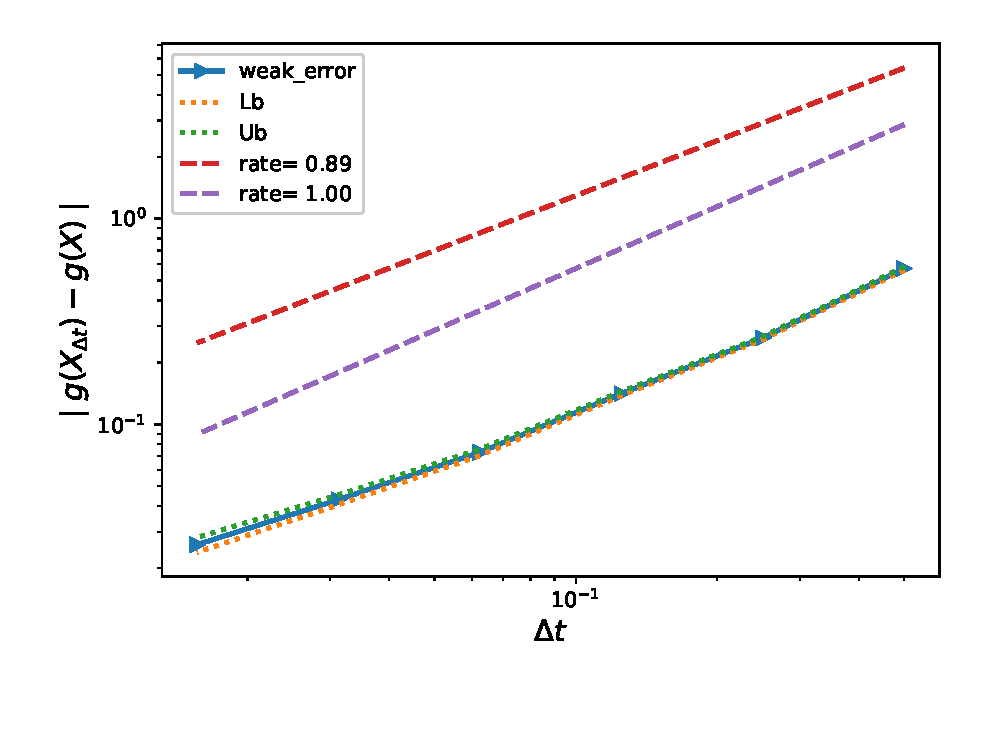
\includegraphics[width=0.6\linewidth]{./figures/rBergomi_weak_error_rates/without_richardson/H_007/weak_convergence_order_Bergomi_H_007_K_1_M_10_6_CI_relative}
		
	\caption{The  convergence of the weak error $\mathcal{E}_B(N)$, using MC ($M=10^6$) with hierarchical hybrid scheme, for set $1$ parameter in Table \ref{table:Reference solution, using MC with $500$ time steps, of Call option price under rBergomi model, for different parameter constellation.}. We refer to $C_{\text{RB}}$ as $\expt{g(X)}$, and to $C_{\text{RB}}^{N}$ as  $\expt{g(X_{\Delta t})}$. The upper and lower bounds are $95\%$ confidence intervals.}
	\label{fig:Weak_rate_set1_without_rich_hybrid}
\end{figure}
\FloatBarrier


\FloatBarrier
\begin{figure}[h!]
	\centering
	\begin{subfigure}{.5\textwidth}
		\centering
		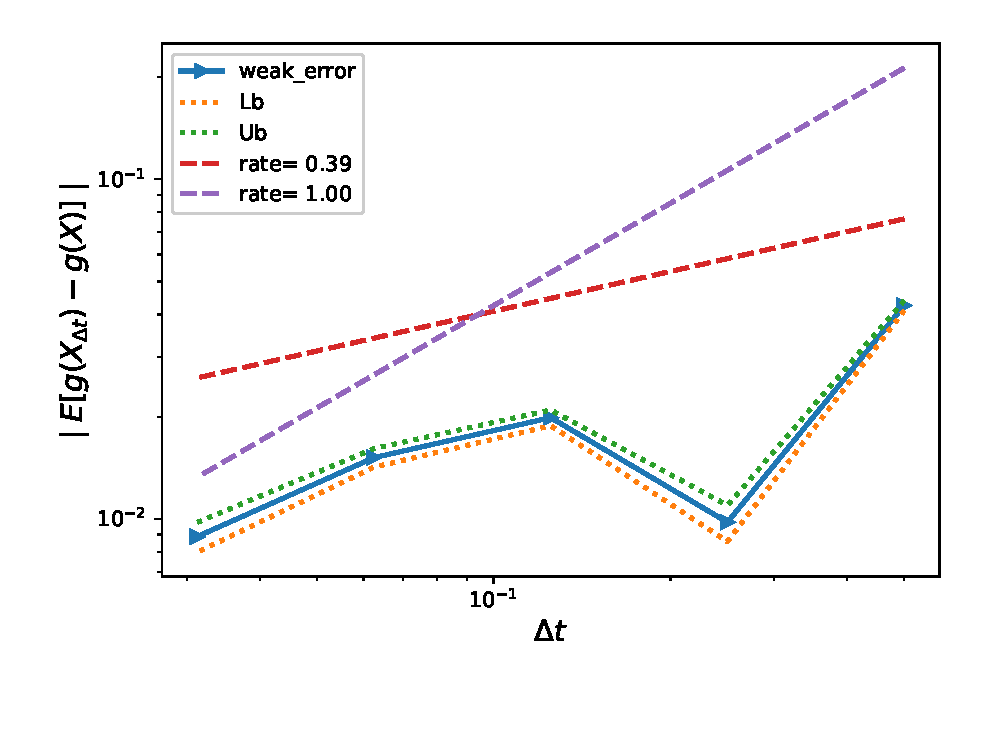
\includegraphics[width=1\linewidth]{./figures/rBergomi_weak_error_cholesky/weak_convergence_order_Bergomi_H_007_K_1_M_6_10_6_CI_relative_cholesky_hierarchical}
		\caption{}
		\label{fig:sub3}
	\end{subfigure}%
	\begin{subfigure}{.5\textwidth}
		\centering
		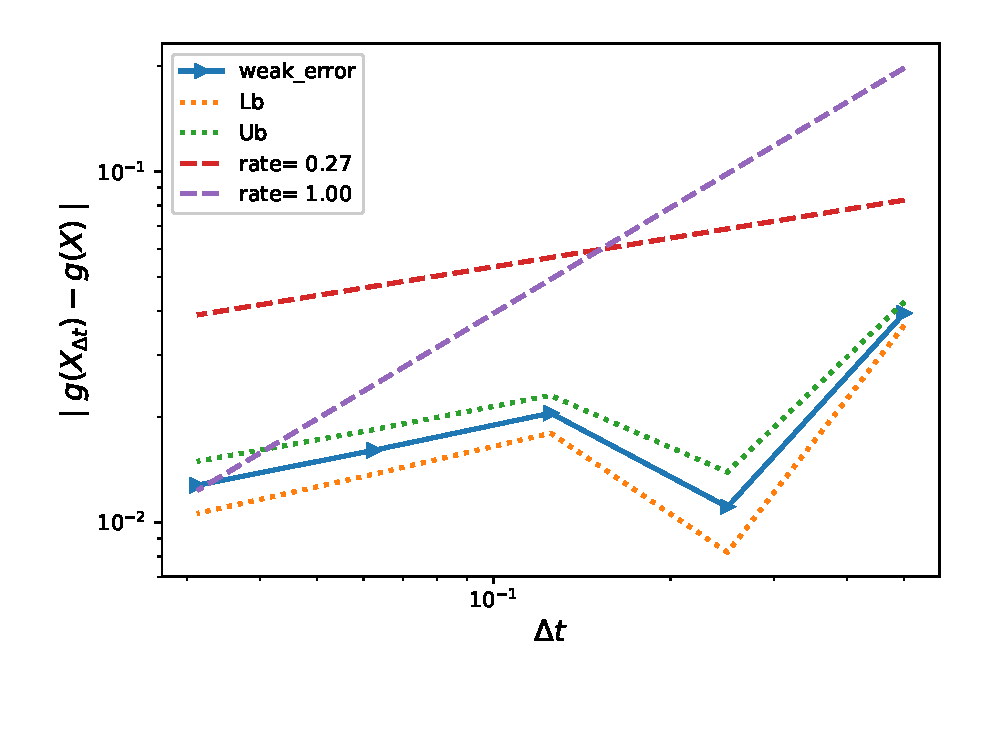
\includegraphics[width=1\linewidth]{./figures/rBergomi_weak_error_cholesky/weak_convergence_order_Bergomi_H_007_K_1_M_10_6_CI_relative_cholesky_non_hierarchical}
		\caption{}
		\label{fig:sub4}
	\end{subfigure}
	
	\caption{The  convergence of the weak error $\mathcal{E}_B(N)$, using MC ($M=6 \times 10^6$) with Cholesky scheme, for set $1$ parameter in Table \ref{table:Reference solution, using MC with $500$ time steps, of Call option price under rBergomi model, for different parameter constellation.}. We refer to $C_{\text{RB}}$ as $\expt{g(X)}$, and to $C_{\text{RB}}^{N}$ as  $\expt{g(X_{\Delta t})}$. The upper and lower bounds are $95\%$ confidence intervals. a) With hierarchical representation.  b) Without hierarchical representation.}
	\label{fig:Weak_rate_set1_set_2_without_rich}
\end{figure}
\FloatBarrier


\FloatBarrier
\begin{figure}[h!]
	\centering
		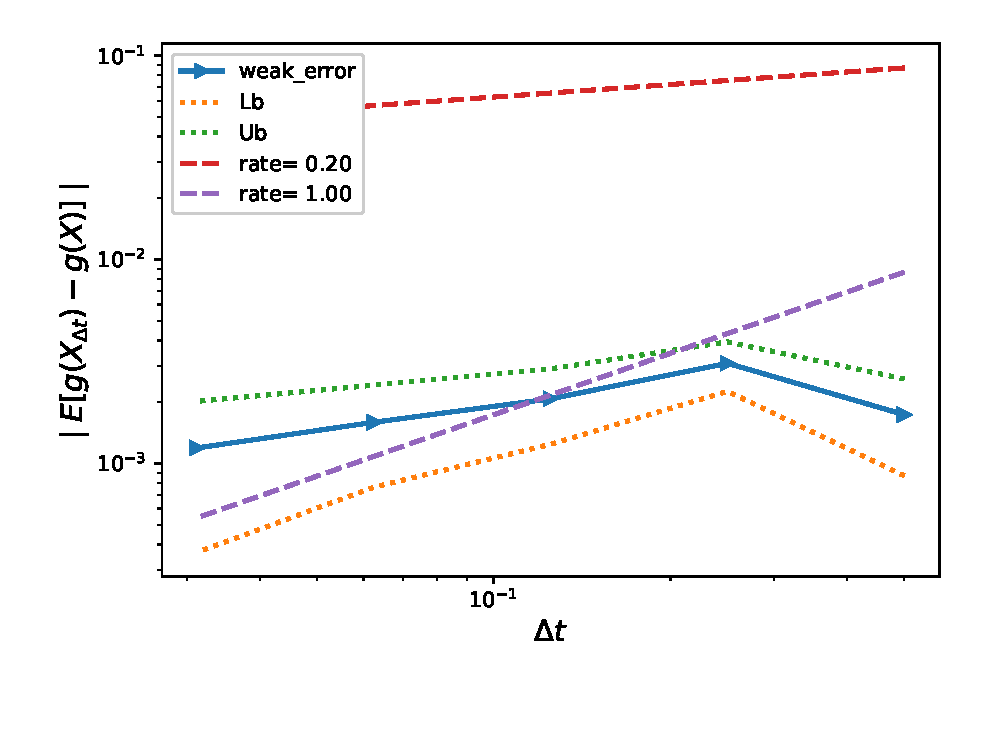
\includegraphics[width=0.6\linewidth]{./figures/rBergomi_weak_error_cholesky/weak_convergence_order_Bergomi_H_002_K_1_M_6_10_6_CI_relative_cholesky_hierarchical}
		
	\caption{The  convergence of the weak error $\mathcal{E}_B(N)$, using MC ($M=6 \times 10^6$) with hierarchical Cholesky scheme, for set $2$ parameter in Table \ref{table:Reference solution, using MC with $500$ time steps, of Call option price under rBergomi model, for different parameter constellation.}. We refer to $C_{\text{RB}}$ as $\expt{g(X)}$, and to $C_{\text{RB}}^{N}$ as  $\expt{g(X_{\Delta t})}$. The upper and lower bounds are $95\%$ confidence intervals.}
	\label{fig:Weak_rate_set2_without_rich_cholesky}
\end{figure}
\FloatBarrier


To investigate more the behavior observed for the Cholesky scheme, we test the case of set $5$ in table \ref{table:Reference solution, using MC with $500$ time steps, of Call option price under rBergomi model, for different parameter constellation.} which is close to the Gaussian case for $H=1/2$ (see Figure \ref{fig:Weak_rate_set1_set_5_without_rich}). We observed a weak convergence rate of order almost $1$. This observation confirms first that maybe the hybrid scheme is more robust, in terms of weak error, than Cholesky for the simulation of the rough Bergomi dynamics. Furthermore, we believe that the weak error in the Cholesky scheme depends on $H$, and  that the common error in both the Cholesky and Hybrid scheme is dominated by the second kind of weak error involved in the hybrid scheme with is of order $\Delta t $ that is why we observed more robust rate for the hybrid scheme. We try in Section \ref{sec:Weak error analysis} to provide an analysis for the weak rate.

\FloatBarrier
\begin{figure}[h!]
	\centering
	\begin{subfigure}{.5\textwidth}
		\centering
		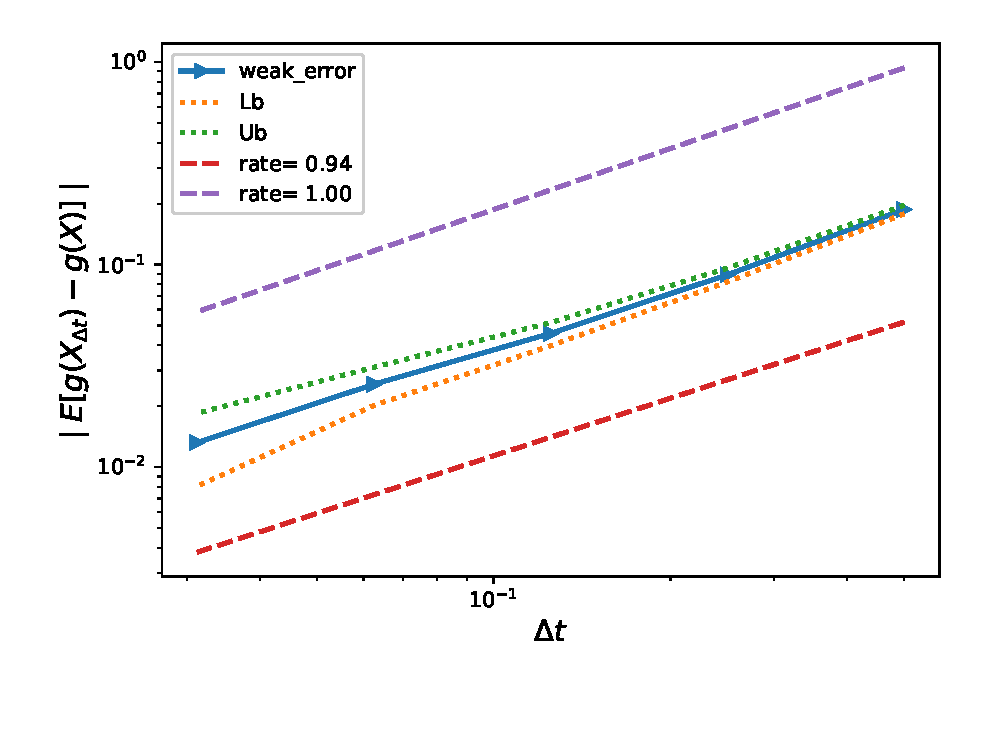
\includegraphics[width=1\linewidth]{./figures/rBergomi_weak_error_cholesky/weak_convergence_order_Bergomi_H_043_K_1_M_10_5_CI_relative_cholesky_hierarchical}
		\caption{}
	\end{subfigure}%
	\begin{subfigure}{.5\textwidth}
		\centering
		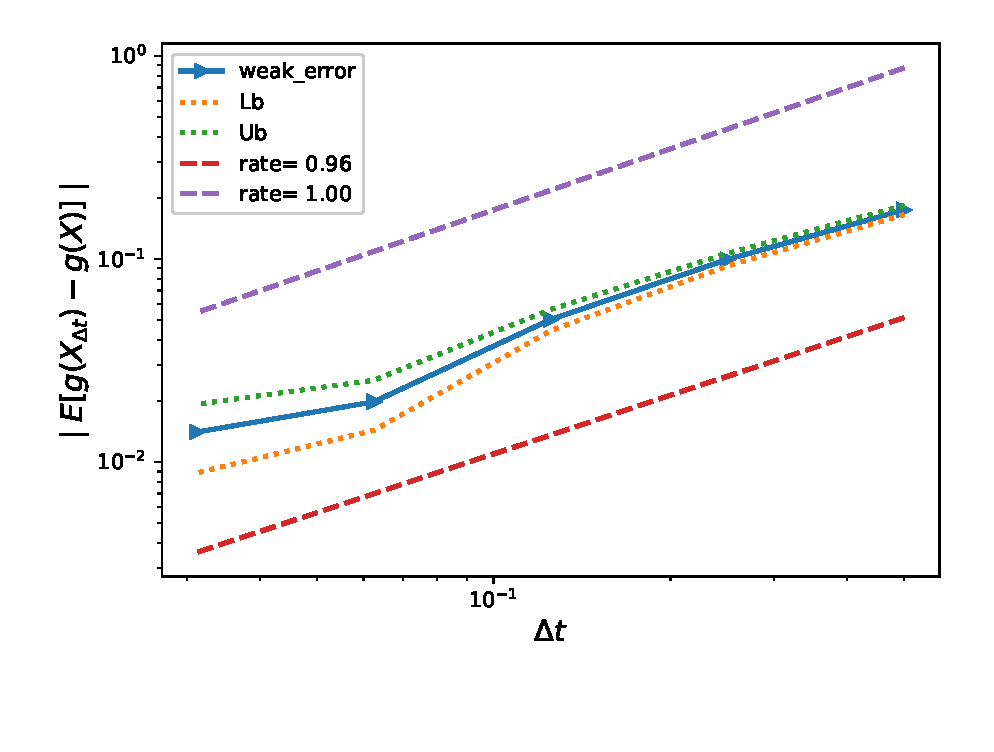
\includegraphics[width=1\linewidth]{./figures/rBergomi_weak_error_cholesky/weak_convergence_order_Bergomi_H_043_K_1_M_10_5_CI_relative_cholesky_non_hierarchical}
		\caption{}
	\end{subfigure}
	
	\caption{The  convergence of the weak error $\mathcal{E}_B(N)$, using MC ($M=10^5$) with Cholesky scheme, for set $5$ parameter in Table \ref{table:Reference solution, using MC with $500$ time steps, of Call option price under rBergomi model, for different parameter constellation.}. We refer to $C_{\text{RB}}$ as $\expt{g(X)}$, and to $C_{\text{RB}}^{N}$ as  $\expt{g(X_{\Delta t})}$. The upper and lower bounds are $95\%$ confidence intervals. a) With hierarchical representation.  b) Without hierarchical representation.}
	\label{fig:Weak_rate_set1_set_5_without_rich}
\end{figure}
\FloatBarrier

\begin{remark}
Our observations are in harmony with results observed in \cite{bayer2017regularity}, where it was observed that the weak error for pricing European option under the rBergomi, simulated using Cholesky scheme and for a particular choice of test function is of order $2H$ across the full range of $0<H <\frac{1}{2}$ (see Figure $3$ in \cite{bayer2017regularity}). On the other hand, I suspect  that the results reported in the Master thesis provided by Christian are reported on opposite way, that is the results reported for the hybrid scheme correspond to the Cholesky scheme (to be checked). 
\end{remark}


\subsection{Comparing the different  errors and computational time for MC and MISC for the Cholesky scheme}\label{sec:Comparing different  errors and complexity for MC and MISC_ Cholesky}
Due to the behavior of the weak error for small values of $H$, we can not apply Richardson extrapolation. However, since the weak error when using Cholesky scheme seems to be one order smaller than the one obtained when using the hybrid scheme, we try to compare the numerical complexity of MC and MISC for the case of set $1$ parameter in Table \ref{table:Reference solution, using MC with $500$ time steps, of Call option price under rBergomi model, for different parameter constellation.}, without using Richardson extrapolation. From Tables \ref{Total error of MISC and MC to compute Call option price of the different tolerances for different number of time steps_Cholesky. Case $K=1$, $H=0.07$, without Richardson extrapolation. The numbers between parentheses are the corresponding absolute errors,linear} and \ref{Comparsion of the computational time of  MC and MISC, used to compute Call option price of rBergomi model_cholesky for different number of time steps. Case $K=1, H=0.07$, linear}, we see that to get a total relative error below $1\%$, we need more than $32$ time steps for both MC and MISC, implying (given our previous results with the hybrid scheme) that using the hybrid scheme coupled with Richardson extrapolation gives better results for MC and MISC, than those obtained with Cholesky scheme.
\FloatBarrier

\begin{table}[h!]
	\centering
	\begin{tabular}{l*{6}{c}r}
	\toprule[1.5pt]
	Method & & Steps  & & &    \\
	\hline
		    & $2$ & $4$ & $8$  & $16$   & $32$ \\
		\hline

		MISC ($\text{TOL}_{\text{MISC}}=10^{-1}$)  & $\underset{(0.042,0.080)}{\mathbf{0.122}}$& $ \underset{(0.010,0.083)}{\mathbf{0.093}}$ & $ \underset{(0.020,0.173)}{\mathbf{0.193}}$   & $ \underset{(0.015,0.135)}{\mathbf{  0.150}}$  &$-$ \\

		MISC ($\text{TOL}_{\text{MISC}}=10^{-2}$)  & $\underset{(0.042,0.080)}{\mathbf{ 0.122}}$ & $ \underset{(0.010,0.006)}{\mathbf{\red{0.016}}}$ & $\underset{(0.020,0.008)}{\mathbf{ \red{0.028}  }}$&  $ \underset{(0.015,0.014)}{\mathbf{\red{0.029}}}$ &$-$ \\
		MISC ($\text{TOL}_{\text{MISC}}=5.10^{-3}$)  & $\underset{(0.042,0.015)}{\mathbf{ \red{0.057}}}$ & $ \underset{(0.010,0.003)}{\mathbf{0.013 }}$ & $-$&  $-$&$-$  \\

				\hline
				MC    & $\underset{(0.042,0.042)}{\mathbf{0.084}}$  & $\underset{(0.010,0.010)}{\mathbf{0.020}}$  &$\underset{(0.020,0.019)}{
				\mathbf{0.039}}$& $\underset{(0.015,0.015)}{
				\mathbf{0.030}}$ &$\underset{(0.009,0.008)}{
				\mathbf{0.017}}$\\	
		M(\# MC samples)   & $10^3$  & $3 \times 10^4$  &$4 \times 10^3$  & $6 \times 10^3$  & $2 \times 10^4$\\
		\bottomrule[1.25pt]
	\end{tabular}
	\caption{Total relative error of MISC, without Richardson extrapolation, with different tolerances, and MC to compute the call option prices for different numbers of time steps, where the rBergomi dynamics are simulated using Cholesky scheme. The values between parentheses correspond to the different errors contributing to the total relative error: for MISC we report the bias and quadrature errors and for MC we report the bias and the statistical errors estimates.}
	\label{Total error of MISC and MC to compute Call option price of the different tolerances for different number of time steps_Cholesky. Case $K=1$, $H=0.07$, without Richardson extrapolation. The numbers between parentheses are the corresponding absolute errors,linear}
\end{table}
\FloatBarrier




\begin{table}[htbp]
	\centering
	\begin{tabular}{l*{6}{c}r}
		\toprule[1.5pt]
	Method & & Steps  & &  &    \\
	\hline
	        & $2$ & $4$ & $8$  &$16$  &$32$ \\
		\hline
		MISC ($\text{TOL}_{\text{MISC}}=10^{-1}$)  & $0.1$ & $0.08$ & $8$  & $670$  &  $-$\\\
		MISC ($\text{TOL}_{\text{MISC}}=10^{-2}$)  & $0.1$ & $\red{2.5}$ & $\red{15}$ &  $\red{2040}$ &  $-$\\\
				MISC ($\text{TOL}_{\text{MISC}}=5.10^{-3}$)  & $\red{0.3}$& $10$ & $-$ &  $-$ &  $-$\\
		\hline	
		MC method & $0.2$  & $5.6$  & $0.8$ & $1.6$  & $22$\\
		\bottomrule[1.25pt]	
		\hline
	\end{tabular}
	\caption{Comparison of the computational time (in seconds) of  MC and MISC, to compute the call option price of the rBergomi model, simulated using Cholesky scheme, for different numbers of time steps. The average MC CPU time is computed over $100$ runs.}
	\label{Comparsion of the computational time of  MC and MISC, used to compute Call option price of rBergomi model_cholesky for different number of time steps. Case $K=1, H=0.07$, linear}
\end{table}
\FloatBarrier
\section{Weak error analysis}\label{sec:Weak error analysis}

To the best of our knowledge, no proper weak error
analysis has been done in the rough volatility context. However, we try in this Section  to shortly discuss it in the context of the rBergomi model.

In this work, we are interested in approximating $\expt{g(X_T)}$, where $g$ is some smooth function and $X$ is the asset price under the rBergomi dynamics such that $X_t=X_t(W^{(1)}_{[0,t]},\widetilde{W}_{[0,t]})$\red{,} where $W^{(1)}$ is standard Brownian motion and  $\widetilde{W}$ is the fractional Brownian motion as given by \eqref{eq:Volterra process}.  Then we can express the approximation of $\expt{g(X_T)}$  using the  hybrid and exact schemes as the following 
\begin{align*}
\expt{g\left(X_T\left(W^{(1)}_{[0,T]},\widetilde{W}_{[0,T]}\right)\right)} \approx \expt{g\left(\overline{X}_N\left(W^{(1)}_1,\dots,W^{(1)}_N, \overline{W}_1, \dots,\overline{W}_N\right)\right)} \quad \textbf{(Hybrid  scheme)},
\end{align*}
\begin{align*}
\expt{g\left(X_T\left(W^{(1)}_{[0,T]},\widetilde{W}_{[0,T]}\right)\right)} \approx \expt{g\left(\overline{X}_N\left(W^{(1)}_1,\dots,W^{(1)}_N, \widetilde{W}_1, \dots,\widetilde{W}_N\right)\right)} \quad \textbf{(Exact  scheme)},
\end{align*}
where $\overline{W}$ is the approximation of $\widetilde{W}$  as given by \eqref{eq:Hybrid_scheme_pre} and $\overline{X}_N$ is the approximation of $X$ using $N$ time steps. In the following, to simplify notation, let  $\overline{\mathbf{W}}=(\overline{W}_1,\dots,\overline{W}_N)$, $\mathbf{W}^{1}=(W^{(1)}_1,\dots,W^{(1)}_N)$ and $\widetilde{\mathbf{W}}=(\widetilde{W}_1,\dots,\widetilde{W}_N)$. Then, the use of Richardson extrapolation in our  methodology presented in Section \ref{sec:Details our approach and error bounds} is mainly justified  by the conjecture \ref{conj: Weak error structure}. 
\begin{conjecture}\label{conj: Weak error structure}
If we denote by $\mathcal{E}_{B}^{\text{Hyb}}$ and $\mathcal{E}_{B}^{\text{Chol}}$ the weak errors produced by the hybrid and Cholesky scheme respectively, then we have
\begin{small}
\begin{align}\label{eq: Weak_error_hyb_chol}
\mathcal{E}_{B}^{\text{Hyb}}&=\abs{\expt{g\left(X_T\left(W^{(1)}_{[0,T]},\widetilde{W}_{[0,T]}\right) \right)}-\expt{g\left(\overline{X}_N\left(\mathbf{W}^{1}, \overline{\mathbf{W}}\right) \right)}} \nonumber\\
&\le \abs{\expt{g\left(X_T\left(W^{(1)}_{[0,T]},\widetilde{W}_{[0,T]}\right)\right)}-\expt{g\left(\overline{X}_N\left(\mathbf{W}^{1}, \widetilde{\mathbf{W}}\right)\right)}}+ \abs{ \expt{g\left(\overline{X}_N\left(\mathbf{W}^{1}, \overline{\mathbf{W}}\right)\right)}- \expt{g\left(\overline{X}_N\left(\mathbf{W}^{1}, \widetilde{\mathbf{W}}\right)\right)}}\nonumber\\
&\le \mathcal{E}_{B}^{\text{Chol}}+ \abs{ \expt{g\left(\overline{X}_N\left(\mathbf{W}^{1}, \overline{\mathbf{W}}\right)\right)}- \expt{g\left(\overline{X}_N\left(\mathbf{W}^{1}, \widetilde{\mathbf{W}}\right)\right)}}.
\end{align}
\end{small}
From the construction of the Cholesky scheme, we expect that the weak error is purely the discretization error, that is
\begin{align*}
\mathcal{E}_{B}^{\text{Chol}}=\Ordo{\Delta t},
\end{align*}
as it was observed by our numerical experiments (for illustration see Figure \ref{fig:set1_weak_rate_exact} for the case of Set $1$  in Table \ref{table:Reference solution, using MC with $500$ time steps, of Call option price under rBergomi model, for different parameter constellation.}).  The second term in the right-hand side of  \eqref{eq: Weak_error_hyb_chol} is basically related to approximating the integral \eqref{eq:Volterra process}  by \eqref{eq:Hybrid_scheme}. From our numerical experiments it seems that this term is  at least  of order  $\Delta t$  and its rate of convergence is independent of $H$ (for illustration see Figure \ref{fig:set1_weak_rate_hybrid} for the case of Set $1$  in Table \ref{table:Reference solution, using MC with $500$ time steps, of Call option price under rBergomi model, for different parameter constellation.}).
\end{conjecture}


 %%%%%%%%%%%%%%%%%%%%%%%%%%%%%%%%%%%%%%%%%%
%References
%%%%%%%%%%%%%%%%%%%%%%%%%%%%%%%%%%%%%%%%%%

\bibliographystyle{plain}
\bibliography{smoothing_rBergomi.bib} 







 

 

 
 
 


\end{document}